

%!TEX root = /Users/kevin/SkyDrive/KTH Work/Period 3 2014/DN2255/Homework/4/HW4-High Resolution shock-capturing methods/HW4_High_Resolution_shock_capturing_methods.tex
\subsubsection{Smooth Steady state solutions} 

% (fold)
\label{subsub:smooth_steady_state_solutions}

% subsubsection smooth_steady_state_solutions (end)
Figure~\ref{fig:Figures_steadySolutionsp1_n_is_80_a_0} shows the plot with the source term 
\begin{equation}
	B(x) = 
	\begin{cases}
		B_0 \cos \left( \frac{\pi(x-L/2)}{2r} \right), &\text{ if }|x-L/2|<r\\
		0, &\text{ if }|x-L/2|>r 
	\end{cases}
	\label{eq:bxEquation} 
\end{equation}

% (eq:bxequation)
\begin{figure}
	[htbp] \centering 
	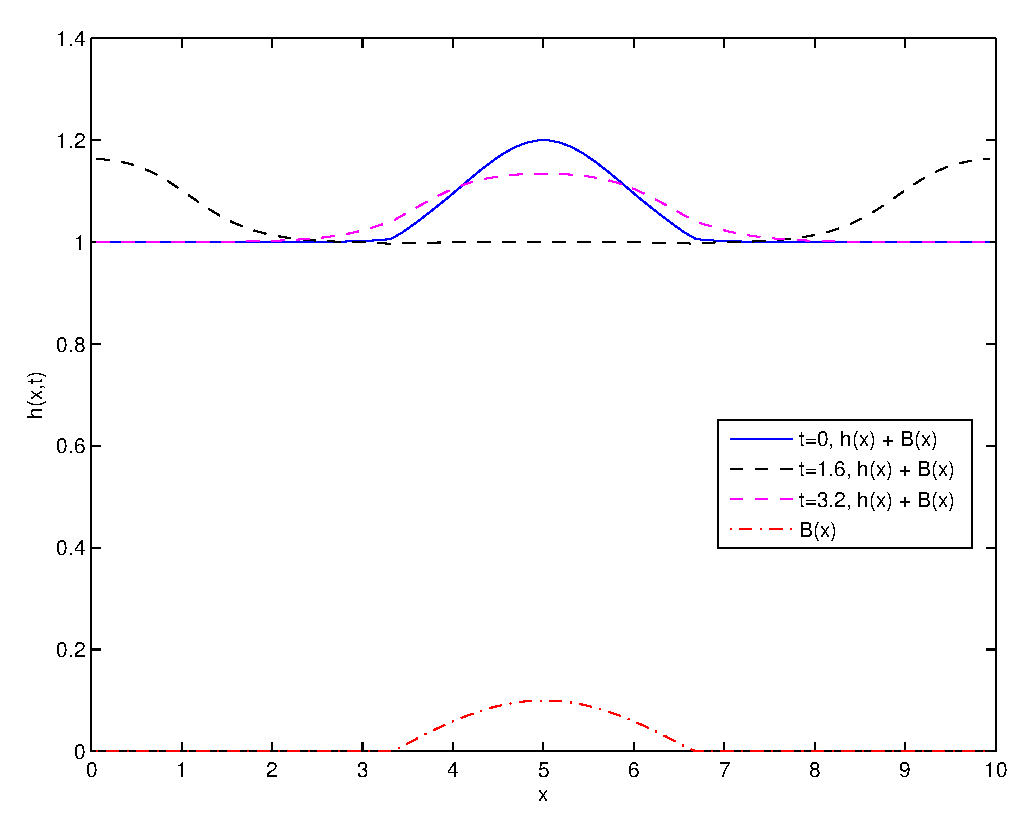
\includegraphics[width=\MyWidth]{Figures/steadySolutionsp1_n_is_80_a_0.eps} \caption{Solution with an uneven bottom that contributes to the wave shape and speed. The depth of the wave is is related to the bottom surface as well as its own surface.} \label{fig:Figures_steadySolutionsp1_n_is_80_a_0} 
\end{figure}

%(fig:Figures_steadySolutionsp1_n_is_80_a_0)
\begin{figure}
	[htbp] \centering 
	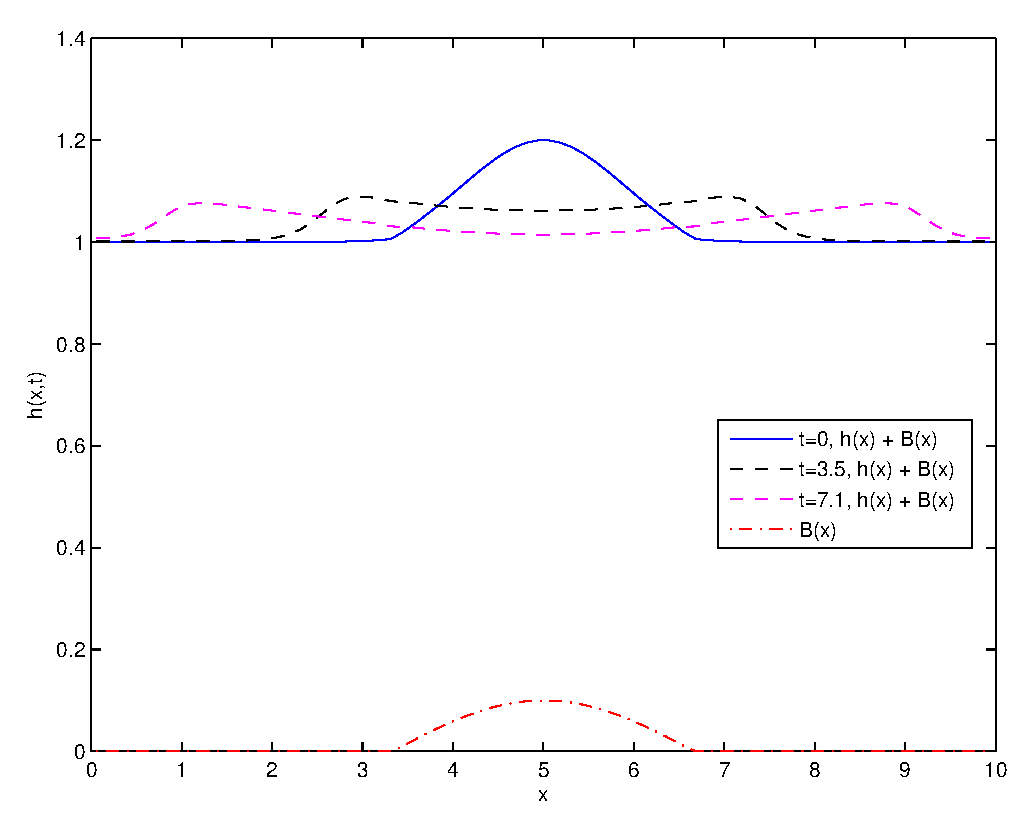
\includegraphics[width=\MyWidth]{Figures/critical_c2817_p1_n_is_80_a_0.eps} \caption{Subcritical condition} \label{fig:Figures_critical_c2817_p1_n_is_80_a_0} 
\end{figure}

%(fig:Figures_critical_c2817_p1_n_is_80_a_0)
\begin{figure}
	[htbp] \centering 
	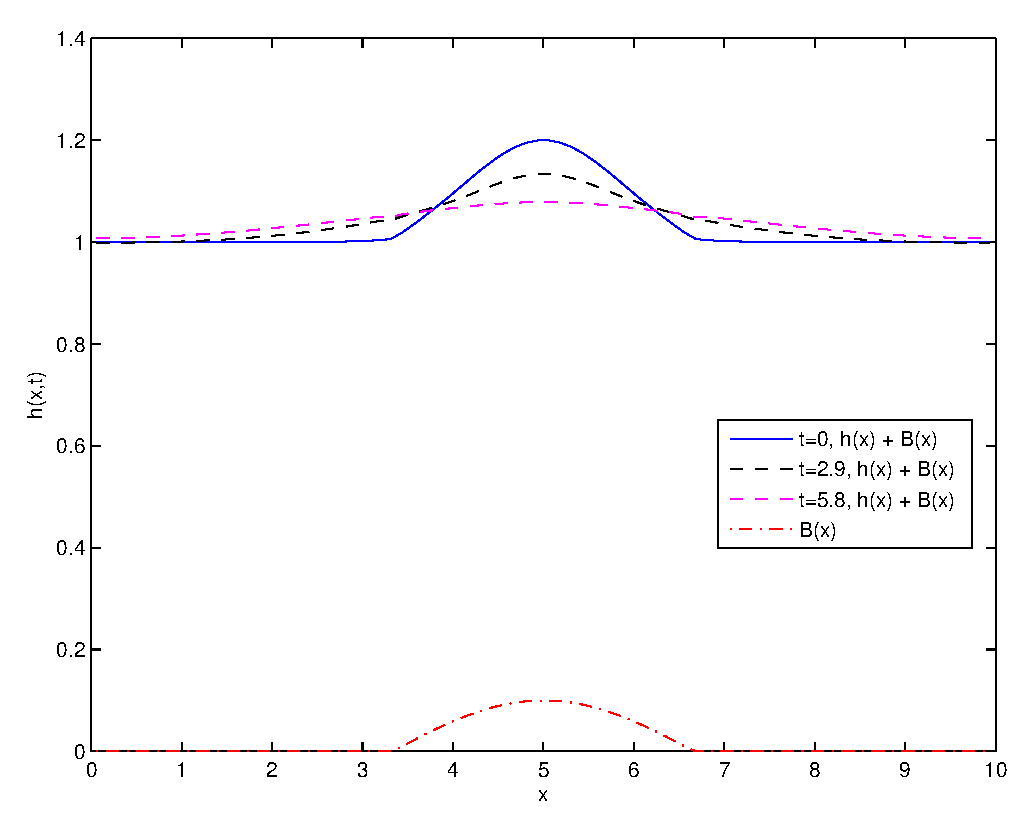
\includegraphics[width=\MyWidth]{Figures/critical_c3444_p1_n_is_80_a_0.eps} \caption{Super-critical} \label{fig:Figures_critical_c3444_p1_n_is_80_a_0} 
\end{figure}

%(fig:Figures_critical_c3444_p1_n_is_80_a_0)
